\documentclass{standalone}
\usepackage{tikz}
\usepackage{ctex,siunitx}
\usepackage{tkz-euclide}
\usepackage{amsmath}
\usetikzlibrary{patterns, calc}
\usetikzlibrary {decorations.pathmorphing, decorations.pathreplacing, decorations.shapes,}
\begin{document}
\small
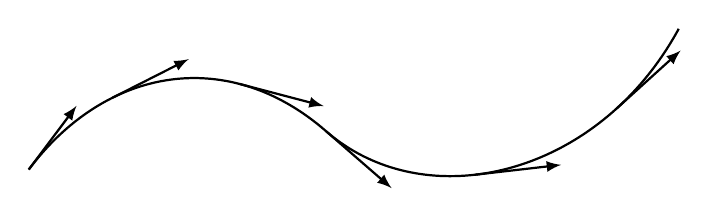
\begin{tikzpicture}[>=latex,thick,scale=1.1]
  % \useasboundingbox (-0.1,0.1) rectangle(6.1,-3.1);
  \draw (0.000, 0.000)..controls(0.276, 0.368)and(0.602, 0.645)..(0.955, 0.823)..controls(1.421, 1.059)and(1.934, 1.120)..(2.438, 0.987)..controls(2.780, 0.897)and(3.118, 0.717)..(3.434, 0.441)..controls(3.906, 0.031)and(4.523,-0.132)..(5.152,-0.060)..controls(5.720, 0.005)and(6.298, 0.262)..(6.785, 0.703)..controls(7.060, 0.952)and(7.305, 1.260)..(7.504, 1.625);
  \draw[->](0.000, 0.000)--(0.276*2, 0.368*2);
  \draw[->](0.955, 0.823)--++(0.892, 0.452);
  \draw[->](2.438, 0.987)--++(0.967, -0.254);
  \draw[->](3.434, 0.441)--++(0.755, -0.656);
  \draw[->](5.152,-0.060)--++(0.994, 0.114);
  \draw[->](6.785, 0.703)--++(0.741, 0.671);
  % \draw[->](0,0)--++(0,-0.8)node[right]{$G$};
  % \draw[->](2.4,-0.48)--++(0,-0.8)node[right]{$G$};
  % \draw[->](2.4,-0.48)--++(1.15,-0.46)node[above]{$v$};
\end{tikzpicture}
\end{document}